\documentclass[border=8pt]{standalone}
\usepackage[T1]{fontenc}
\usepackage{mathptmx}
\usepackage{tikz}
\usetikzlibrary{arrows.meta,positioning,fit,calc,shapes.geometric,shapes.misc,shapes.multipart,backgrounds}
\tikzset{
  arr/.style={-{Stealth[length=2.4mm,width=1.8mm]},line width=0.6pt},
  box/.style={draw,line width=0.6pt,align=center,rounded corners=2pt},
}

\begin{document}
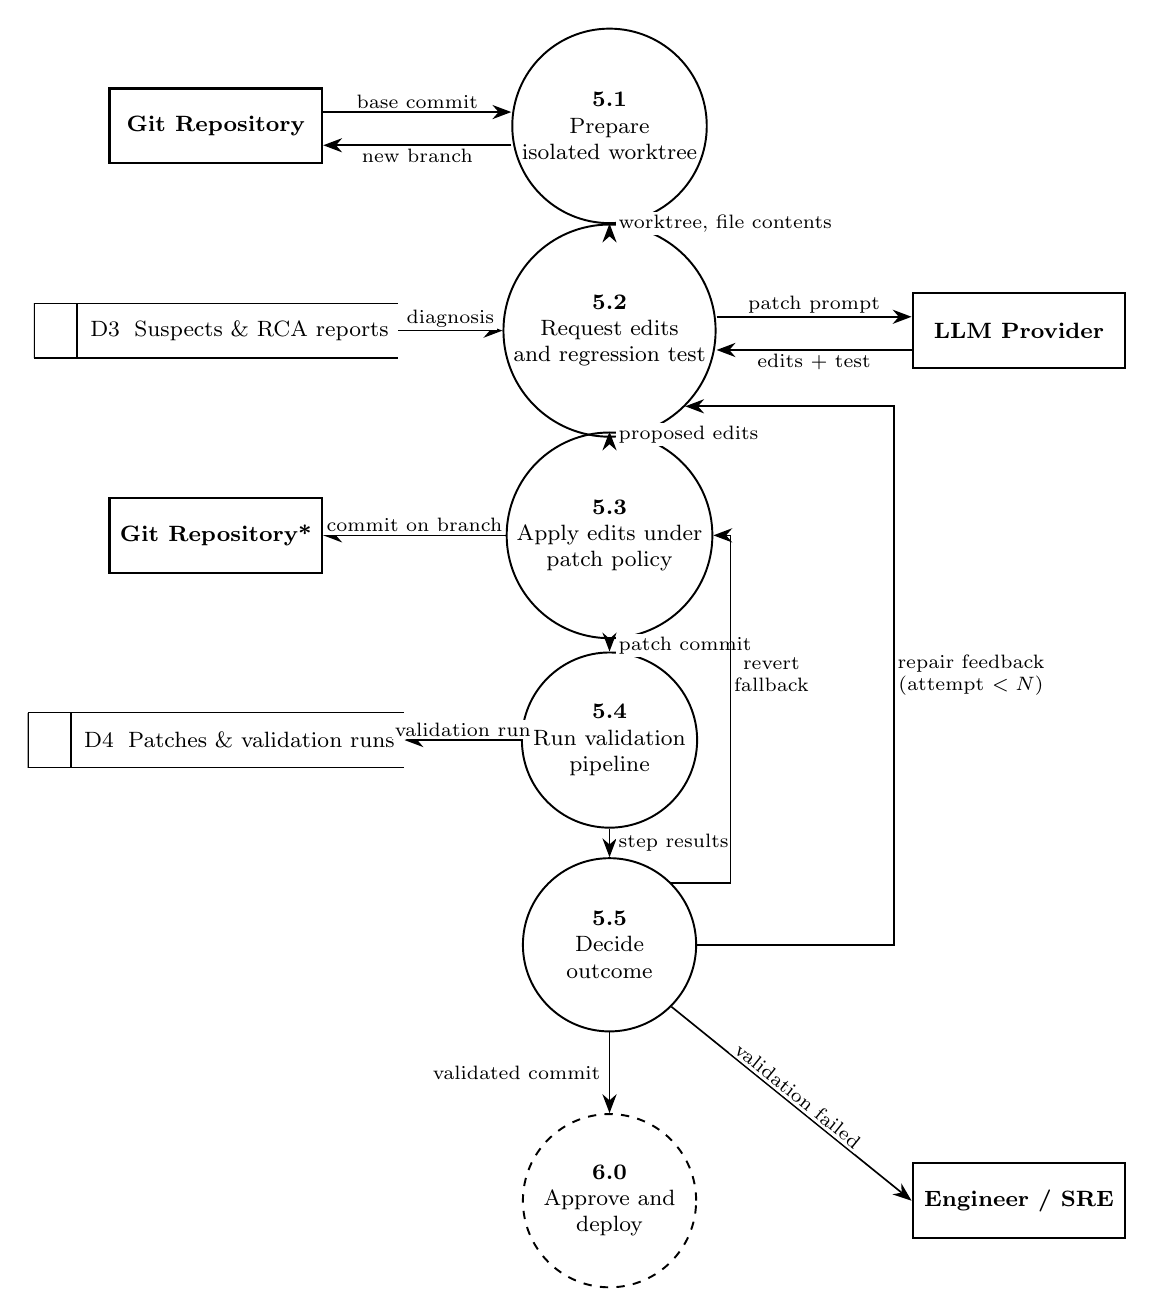
\begin{tikzpicture}[font=\small,
  proc/.style={circle, draw, line width=0.7pt, minimum size=2.2cm, align=center, inner sep=1pt, font=\footnotesize},
  ent/.style={draw, line width=0.8pt, minimum width=2.7cm, minimum height=0.95cm, align=center, font=\footnotesize\bfseries},
  store/.style={draw=none, minimum width=3.3cm, minimum height=0.7cm, align=left, font=\footnotesize, path picture={
     \draw[line width=0.7pt] (path picture bounding box.north west) -- (path picture bounding box.north east);
     \draw[line width=0.7pt] (path picture bounding box.south west) -- (path picture bounding box.south east);
     \draw[line width=0.7pt] (path picture bounding box.north west) -- (path picture bounding box.south west);
     \draw[line width=0.7pt] ([xshift=0.55cm]path picture bounding box.north west) -- ([xshift=0.55cm]path picture bounding box.south west);}},
  lab/.style={font=\scriptsize, fill=white, inner sep=1pt, align=center}]
\def\dy{2.6}
\node[proc] (p1) at (0,0) {\textbf{5.1}\\ Prepare\\ isolated worktree};
\node[proc] (p2) at (0,-\dy) {\textbf{5.2}\\ Request edits\\ and regression test};
\node[proc] (p3) at (0,-2*\dy) {\textbf{5.3}\\ Apply edits under\\ patch policy};
\node[proc] (p4) at (0,-3*\dy) {\textbf{5.4}\\ Run validation\\ pipeline};
\node[proc] (p5) at (0,-4*\dy) {\textbf{5.5}\\ Decide\\ outcome};
\node[proc, dashed] (p6) at (0,-5.25*\dy) {\textbf{6.0}\\ Approve and\\ deploy};
\node[ent] (git) at (-5.0,0) {Git Repository};
\node[store] (d3) at (-5.0,-\dy) {\hspace{0.55cm}\,D3\; Suspects \& RCA reports};
\node[ent] (git2) at (-5.0,-2*\dy) {Git Repository*};
\node[store] (d4) at (-5.0,-3*\dy) {\hspace{0.55cm}\,D4\; Patches \& validation runs};
\node[ent] (llm) at (5.2,-\dy) {LLM Provider};
\node[ent] (eng) at (5.2,-5.25*\dy) {Engineer / SRE};
\draw[arr] (p1) -- node[lab, right=2pt] {worktree, file contents} (p2);
\draw[arr] (p2) -- node[lab, right=2pt] {proposed edits} (p3);
\draw[arr] (p3) -- node[lab, right=2pt] {patch commit} (p4);
\draw[arr] (p4) -- node[lab, right=2pt] {step results} (p5);
\draw[arr] (p5) -- node[lab, left=2pt] {validated commit} (p6);
\draw[arr] ([yshift=5pt]git.east) -- node[lab, above] {base commit} ([yshift=5pt]p1.west);
\draw[arr] ([yshift=-7pt]p1.west) -- node[lab, below] {new branch} ([yshift=-7pt]git.east);
\draw[arr] (d3.east) -- node[lab, above] {diagnosis} (p2.west);
\draw[arr] (p3.west) -- node[lab, above] {commit on branch} (git2.east);
\draw[arr] (p4.west) -- node[lab, above] {validation run} (d4.east);
\draw[arr] ([yshift=5pt]p2.east) -- node[lab, above] {patch prompt} ([yshift=5pt]llm.west);
\draw[arr] ([yshift=-7pt]llm.west) -- node[lab, below] {edits + test} ([yshift=-7pt]p2.east);
\draw[arr] (p5.east) -- ++(2.5,0) |- node[lab, pos=0.25, right] {repair feedback\\(attempt $<N$)} (p2.south east);
\draw[arr] (p5.north east) -- ++(0.75,0) |- node[lab, pos=0.3, right] {revert\\ fallback} (p3.east);
\draw[arr] (p5.south east) -- node[lab, sloped, above] {validation failed} (eng.west);
\end{tikzpicture}
\end{document}
